\documentclass[12pt]{article}
\usepackage[utf8]{inputenc}
\usepackage{graphicx} 
\usepackage{wrapfig}
\usepackage[dvipsnames]{xcolor}
\usepackage{moreverb}
\usepackage{ragged2e}
\renewcommand\refname{Referencias}
\title{Elementos de la programación Python 1.}
\author{\textcolor{JungleGreen}{Olga María Fimbres Morales}}
\date{17 de Enero 2016}
\begin{document}
\begin{titlepage}

\begin{center}
\begin{large}
Universidad del Estado de Sonora\\
\end{large}
\vspace*{0.15in}
División de Ciencias Exactas y Naturales.\\
\vspace*{0.15in}
Licenciatura en Física. \\
\vspace*{0.6in}
\begin{large}
Física Computacional 1\\
\end{large}
\vspace*{0.2in}
\begin{Large}
\textbf{{\textcolor{Red}{Aproximación al cálculo del periodo del péndulo.}}} \\
\end{Large}

%\begin{Large}
%\textbf{{\textcolor{Red}{Péndulo.}}} \\
%end{Large}
%\vspace*{-1in}

\rule{80mm}{0.1mm}\\
\vspace*{0.1in}
\begin{large}
{\textcolor{JungleGreen}{Olga María Fimbres Morales}}\\
1 de Mayo de 2016\\
\end{large}
\end{center}
\end{titlepage}

\pagebreak
\section*{Introducción.}
 Retomamos nuevamente el modelo de péndulo como tema de estudio, esta vez utilizando nuestra nueva herramienta, Maxima, para desarrollar un mejor calculo que el realizado en una actividad anterior sobre el periodo del péndulo y el error relativo que este posee dependiendo del método que se utilice para encontrarlo.\\
 
 Como ya se menciono, utilizaremos Maxima para llegar a la expresión del periodo por medio de una serie de Taylor, evidenciando de esta forma que es posible conseguir una mejor estimación del mismo por medio de herramientas computacionales que una vez comprendidas y sabiéndolas utilizar pueden ser de gran utilidad en el momento en que deseamos un calculo mucho más exacto, aspecto que beneficia nuestras investigaciones y trabajos.\\
 
 Se muestra la forma en que se desarrolló esto con, además de una gráfica que muestra errores relativos del periodo para diferentes ángulos utilizando un proceso de aproximación por medio del método de potencias.
 
 
\section*{\textcolor{Red}{Desarrollo en serie.}}

Sabemos que una forma de obtener un mejor calculo o una mejor aproximación al valor real de un parámetro es por medio de un desarrollo en serie, en este caso utilizamos principalmente un desarrollo por medio de series de Taylor; que como sabemos es una aproximaciones de funciones por medio de una suma de potencias para un determinado valor, que debe ser suficientemente derivable sobre la función y un entorno sobre el cual converja a la serie.\\

También podemos hablar de las series de Maclaurin, las cuales son series de Taylor de una función iniciando desde el cero; además de que son un tipo de expansión en la cual sus términos son potencias no negativas enteras de la variable.

\pagebreak
\section*{\textcolor{LimeGreen}{Problema.}}

Con el fin de poner en práctica una parte de lo aprendido en la actividad anterior buscamos tener una mayor interacción con la forma de trabajar de Maxima, siendo la mejor opción para hacerlo el utilizar sus herramientas con el fin de llegar a una expresión determinada.\\

En esta actividad se nos pide demostrar que es posible expresar el periodo de un péndulo por medio de una serie de Maclaurin; lo cual logramos con el desarrollo de series de Taylor. con que cuenta Maxima.\\

Además de esto se pide desarrollar una gráfica de el error relativo de los periodos de péndulos para diferentes ángulos por medio del método de potencias, como lo son los anteriormente mencionados.\\

Inicialmente se definió la expresión a desarrollar:

\noindent
%%%%%%%%%%%%%%%
%%% INPUT:
\begin{minipage}[t]{8ex}{\color{red}\bf
\begin{verbatim}
(%i1) 
\end{verbatim}}
\end{minipage}
\begin{minipage}[t]{\textwidth}{\color{blue}
\begin{verbatim}
(1/sqrt(1-k^2*sin(x)^2));
\end{verbatim}}
\end{minipage}
%%% OUTPUT:
\definecolor{labelcolor}{RGB}{100,0,0}
\begin{math}\displaystyle
\parbox{8ex}{\color{labelcolor}(\%o1) }
\frac{1}{\sqrt{1−{k}^{2}\,{\mathrm{sin}\left( x\right) }^{2}}}
\end{math}
%%%%%%%%%%%%%%%

La cual se desarrolló por medio de una serie de Taylor hasta la octava potencia:
\begin{center}
\begin{minipage}[t]{\textwidth}{\color{blue}
\begin{verbatim}
B : taylor((1/sqrt(1-k^2*sin(x)^2)), x, 0, 8);
\end{verbatim}}
\end{minipage}
%%% OUTPUT:
\definecolor{labelcolor}{RGB}{100,0,0}
\begin{math}\displaystyle
\parbox{8ex}{\color{labelcolor}(\%o3)/T/ }
1+\frac{{k}^{2}\,{x}^{2}}{2}+\frac{\left( 9\,{k}^{4}−4\,{k}^{2}\right) \,{x}^{4}}{24}+\frac{\left( 225\,{k}^{6}−180\,{k}^{4}+16\,{k}^{2}\right) \,{x}^{6}}{720}\\
+\frac{\left( 11025\,{k}^{8}−12600\,{k}^{6}+3024\,{k}^{4}−64\,{k}^{2}\right) \,{x}^{8}}{40320}+...
\end{math}
\end{center}
%%%%%%%%%%%%%%%

Esta expresión es la que se trabajo durante todo el proceso, aplicando extensiones y contracciones de la misma por medio de diversos procesos; inicialmente se busco especificar cada uno de los cocientes que acompañaban a cada potencia de la variable para después desarrollar de una manera mucho mas ordenada y compacta, sin embargo esto no resulto muy conveniente pues era necesario aplicarlo múltiples veces hasta obtener algo cercano a una reducción. Por lo que se optó por seguir un nuevo camino donde sin definir coeficientes de desarrolló la integración de la expresión para después expandirla y de esta forma obtener una expresión mucho más ordenada.\\

Puede verse que después es definida la variable $K(\theta) = \sin(\theta)$ que más tarde sera sustituida dentro de nuestra serie. Para finalmente por medio de factorizaciones se llega a la forma deseada de la expresión del periodo de un péndulo; que más tarde podrá ser utilizada para calcular diferentes periodos simplemente suministrando las variables requeridas.. La secuencia completa, incluyendo los primeros pasos erróneos serán agregados a los anexos.\\

Además de esto, se nos pide calcular el periodo por medio de la expresión:\\


\noindent
%%%%%%%%%%%%%%%
%%% INPUT:
\begin{minipage}[t]{8ex}{\color{red}\bf
\begin{verbatim}
(%i3) 
\end{verbatim}}
\end{minipage}
\begin{minipage}[t]{\textwidth}{\color{blue}
\begin{verbatim}
define(T(%theta), (%));
\end{verbatim}}
\end{minipage}
%%% OUTPUT:
\definecolor{labelcolor}{RGB}{100,0,0}
\begin{math}\displaystyle
\parbox{8ex}{\color{labelcolor}(\%o3) }
\mathrm{T}\left( \theta\right) :=2\,\pi \,\sqrt{\frac{l}{g}}\,\sum_{n=0}^{\infty }\frac{{\mathrm{sin}\left( \frac{\theta}{2}\right) }^{2\,n}\,\left( 2\,n\right) !}{{2}^{2\,n}\,{n!}^{2}}
\end{math}\\
%%%%%%%%%%%%%%%

Evaluar para distintas potencias y conocer el error relativo de este periodo para finalmente graficar. Para ello se genero un código en Python que nos permitiera realizar un ciclo de evaluaci\'on para diferentes casos, realizar el cociente con el periodo teórico que ya conocemos y terminar graficando los casos juntos.\\

Podemos ver que la forma de calcular un solo caso sera igual a todos los demás, simplemente cambiamos el parámetro de las potencias.

\begin{boxedverbatim}
# Parametros
g = 9.806
l = 1.00
n = 200
radtodeg = 180.0/np.pi
epsilon = 0.001
# Secuencia angulo incial
theta_cero = np.linspace(epsilon, np.pi -epsilon, n) 

# Arreglos
integral     = [0 for i in range(n)]
integral0     = [0 for i in range(n)]
err         = [0 for i in range(n)]
perio_num     = [0 for i in range(n)]
sine         = [0 for i in range(n)]
caso0         = [0 for i in range(n)]

# Definir la funcion a integrar: x - variable de int, y - param
# func = lambda x, k : 1.0 /(np.sqrt(np.cos(x)-np.cos(k)))


# Periodo aproximado con la ec. para angulos chicos
pert = 2.0*np.pi*np.sqrt(l/g)

m = 0
for i in range(0,m):
    for j in range(0,n):
        fac1 = float(math.factorial(2*(i)))
        fac2 = float((2**(i) * math.factorial(i))**2)
        sine[j] = np.sin(theta_cero[j]/2)**(2*(i))
        integral[j] = ((fac1/fac2)**2)*sine[j]
        integral0[j] = integral0[j] + integral[j]
        pernum[j] = 2.0*np.pi*np.sqrt(l/g)*integral0[j]
        caso0[j] = pernum[j]/pert 
\end{boxedverbatim}







\pagebreak

\section*{\textcolor{RoyalBlue}{Resultados}}

Desarrollo para llegar a la expresión del periodo del péndulo:



\noindent
%%%%%%%%%%%%%%%
%%% INPUT:
\begin{minipage}[t]{8ex}{\color{red}\bf
\begin{verbatim}
(%i17) 
\end{verbatim}}
\end{minipage}
\begin{minipage}[t]{\textwidth}{\color{blue}
\begin{verbatim}
/*Secuencia correcta*/
B : taylor((1/sqrt(1-k^2*sin(x)^2)), x, 0, 6);
\end{verbatim}}
\end{minipage}
%%% OUTPUT:
\definecolor{labelcolor}{RGB}{100,0,0}
\begin{math}\displaystyle
\parbox{8ex}{\color{labelcolor}(\%o17)/T/ }
1+\frac{{k}^{2}\,{x}^{2}}{2}+\frac{\left( 9\,{k}^{4}−4\,{k}^{2}\right) \,{x}^{4}}{24}+\frac{\left( 225\,{k}^{6}−180\,{k}^{4}+16\,{k}^{2}\right) \,{x}^{6}}{720}+...
\end{math}
%%%%%%%%%%%%%%%

\noindent
%%%%%%%%%%%%%%%
%%% INPUT:
\begin{minipage}[t]{8ex}{\color{red}\bf
\begin{verbatim}
(%i18) 
\end{verbatim}}
\end{minipage}
\begin{minipage}[t]{\textwidth}{\color{blue}
\begin{verbatim}
integrate(B,x,0,%pi/2);
\end{verbatim}}
\end{minipage}
%%% OUTPUT:
\definecolor{labelcolor}{RGB}{100,0,0}
\begin{math}\displaystyle
\parbox{8ex}{\color{labelcolor}(\%o18) }
\frac{225\,{\pi }^{7}\,{k}^{6}+\left( 1512\,{\pi }^{5}−180\,{\pi }^{7}\right) \,{k}^{4}+\left( 16\,{\pi }^{7}−672\,{\pi }^{5}+13440\,{\pi }^{3}\right) \,{k}^{2}+322560\,\pi }{645120}
\end{math}
%%%%%%%%%%%%%%%

\noindent
%%%%%%%%%%%%%%%
%%% INPUT:
\begin{minipage}[t]{8ex}{\color{red}\bf
\begin{verbatim}
(%i19) 
\end{verbatim}}
\end{minipage}
\begin{minipage}[t]{\textwidth}{\color{blue}
\begin{verbatim}
C : expand(%);
\end{verbatim}}
\end{minipage}
%%% OUTPUT:
\definecolor{labelcolor}{RGB}{100,0,0}
\begin{math}\displaystyle
\parbox{8ex}{\color{labelcolor}(\%o19) }
\frac{5\,{\pi }^{7}\,{k}^{6}}{14336}−\frac{{\pi }^{7}\,{k}^{4}}{3584}+\frac{3\,{\pi }^{5}\,{k}^{4}}{1280}+\frac{{\pi }^{7}\,{k}^{2}}{40320}−\frac{{\pi }^{5}\,{k}^{2}}{960}+\frac{{\pi }^{3}\,{k}^{2}}{48}+\frac{\pi }{2}
\end{math}
%%%%%%%%%%%%%%%

\noindent
%%%%%%%%%%%%%%%
%%% INPUT:
\begin{minipage}[t]{8ex}{\color{red}\bf
\begin{verbatim}
(%i20) 
\end{verbatim}}
\end{minipage}
\begin{minipage}[t]{\textwidth}{\color{blue}
\begin{verbatim}
define(K(%theta),sin(%theta));
\end{verbatim}}
\end{minipage}
%%% OUTPUT:
\definecolor{labelcolor}{RGB}{100,0,0}
\begin{math}\displaystyle
\parbox{8ex}{\color{labelcolor}(\%o20) }
\mathrm{K}\left( \theta\right) :=\mathrm{sin}\left( \theta\right) 
\end{math}
%%%%%%%%%%%%%%%

\noindent
%%%%%%%%%%%%%%%
%%% INPUT:
\begin{minipage}[t]{8ex}{\color{red}\bf
\begin{verbatim}
(%i21) 
\end{verbatim}}
\end{minipage}
\begin{minipage}[t]{\textwidth}{\color{blue}
\begin{verbatim}
D : subst(K(%theta/2),k,C);
\end{verbatim}}
\end{minipage}
%%% OUTPUT:
\definecolor{labelcolor}{RGB}{100,0,0}
\begin{math}\displaystyle
\parbox{8ex}{\color{labelcolor}(\%o21) }
\frac{5\,{\pi }^{7}\,{\mathrm{sin}\left( \frac{\theta}{2}\right) }^{6}}{14336}−\frac{{\pi }^{7}\,{\mathrm{sin}\left( \frac{\theta}{2}\right) }^{4}}{3584}+\frac{3\,{\pi }^{5}\,{\mathrm{sin}\left( \frac{\theta}{2}\right) }^{4}}{1280}+\frac{{\pi }^{7}\,{\mathrm{sin}\left( \frac{\theta}{2}\right) }^{2}}{40320}−\frac{{\pi }^{5}\,{\mathrm{sin}\left( \frac{\theta}{2}\right) }^{2}}{960}+\frac{{\pi }^{3}\,{\mathrm{sin}\left( \frac{\theta}{2}\right) }^{2}}{48}+\frac{\pi }{2}
\end{math}
%%%%%%%%%%%%%%%

\noindent
%%%%%%%%%%%%%%%
%%% INPUT:
\begin{minipage}[t]{8ex}{\color{red}\bf
\begin{verbatim}
(%i22) 
\end{verbatim}}
\end{minipage}
\begin{minipage}[t]{\textwidth}{\color{blue}
\begin{verbatim}
D * 2/%pi;
\end{verbatim}}
\end{minipage}
%%% OUTPUT:
\definecolor{labelcolor}{RGB}{100,0,0}
\begin{math}\displaystyle
\parbox{8ex}{\color{labelcolor}(\%o22) }
\frac{2\,\left( \frac{5\,{\pi }^{7}\,{\mathrm{sin}\left( \frac{\theta}{2}\right) }^{6}}{14336}−\frac{{\pi }^{7}\,{\mathrm{sin}\left( \frac{\theta}{2}\right) }^{4}}{3584}+\frac{3\,{\pi }^{5}\,{\mathrm{sin}\left( \frac{\theta}{2}\right) }^{4}}{1280}+\frac{{\pi }^{7}\,{\mathrm{sin}\left( \frac{\theta}{2}\right) }^{2}}{40320}−\frac{{\pi }^{5}\,{\mathrm{sin}\left( \frac{\theta}{2}\right) }^{2}}{960}+\frac{{\pi }^{3}\,{\mathrm{sin}\left( \frac{\theta}{2}\right) }^{2}}{48}+\frac{\pi }{2}\right) }{\pi }
\end{math}
%%%%%%%%%%%%%%%

\noindent
%%%%%%%%%%%%%%%
%%% INPUT:
\begin{minipage}[t]{8ex}{\color{red}\bf
\begin{verbatim}
(%i23) 
\end{verbatim}}
\end{minipage}
\begin{minipage}[t]{\textwidth}{\color{blue}
\begin{verbatim}
F: expand(%);
\end{verbatim}}
\end{minipage}
%%% OUTPUT:
\definecolor{labelcolor}{RGB}{100,0,0}
\begin{math}\displaystyle
\parbox{8ex}{\color{labelcolor}(\%o23) }
\frac{5\,{\pi }^{6}\,{\mathrm{sin}\left( \frac{\theta}{2}\right) }^{6}}{7168}−\frac{{\pi }^{6}\,{\mathrm{sin}\left( \frac{\theta}{2}\right) }^{4}}{1792}+\frac{3\,{\pi }^{4}\,{\mathrm{sin}\left( \frac{\theta}{2}\right) }^{4}}{640}+\frac{{\pi }^{6}\,{\mathrm{sin}\left( \frac{\theta}{2}\right) }^{2}}{20160}−\frac{{\pi }^{4}\,{\mathrm{sin}\left( \frac{\theta}{2}\right) }^{2}}{480}+\frac{{\pi }^{2}\,{\mathrm{sin}\left( \frac{\theta}{2}\right) }^{2}}{24}+1
\end{math}
%%%%%%%%%%%%%%%

\noindent
%%%%%%%%%%%%%%%
%%% INPUT:
\begin{minipage}[t]{8ex}{\color{red}\bf
\begin{verbatim}
(%i24) 
\end{verbatim}}
\end{minipage}
\begin{minipage}[t]{\textwidth}{\color{blue}
\begin{verbatim}
define(T(%theta), (2*%pi)*(sqrt(l/g))*(F));
\end{verbatim}}
\end{minipage}
%%% OUTPUT:
\definecolor{labelcolor}{RGB}{100,0,0}
\begin{math}\displaystyle
\parbox{8ex}{\color{labelcolor}(\%o24) }
\mathrm{T}\left( \theta\right) :=2\,\pi \,\frac{5\,{\pi }^{6}\,{\mathrm{sin}\left( \frac{\theta}{2}\right) }^{6}}{7168}−\frac{{\pi }^{6}\,{\mathrm{sin}\left( \frac{\theta}{2}\right) }^{4}}{1792}+\frac{3\,{\pi }^{4}\,{\mathrm{sin}\left( \frac{\theta}{2}\right) }^{4}}{640}+\frac{{\pi }^{6}\,{\mathrm{sin}\left( \frac{\theta}{2}\right) }^{2}}{20160}−\frac{{\pi }^{4}\,{\mathrm{sin}\left( \frac{\theta}{2}\right) }^{2}}{480}+\frac{{\pi }^{2}\,{\mathrm{sin}\left( \frac{\theta}{2}\right) }^{2}}{24}+1 \,\sqrt{\frac{l}{g}}
\end{math}
%%%%%%%%%%%%%%%

\noindent
%%%%%%%%%%%%%%%
%%% INPUT:
\begin{minipage}[t]{8ex}{\color{red}\bf
\begin{verbatim}
(%i25) 
\end{verbatim}}
\end{minipage}
\begin{minipage}[t]{\textwidth}{\color{blue}
\begin{verbatim}
l :1;
g :9.8;
float(T(%pi/2));
\end{verbatim}}
\end{minipage}
%%% OUTPUT:
\definecolor{labelcolor}{RGB}{100,0,0}
\begin{math}\displaystyle
\parbox{8ex}{\color{labelcolor}(\%o25) }
1
\end{math}

\begin{math}\displaystyle
\parbox{8ex}{\color{labelcolor}(\%o26) }
9.8
\end{math}

\begin{math}\displaystyle
\parbox{8ex}{\color{labelcolor}(\%o27) }
2.392146754285953
\end{math}\\
%%%%%%%%%%%%%%%

Podemos observar como el proceso resulta sencillo si se esta consiente de las herramientas que se utilizan y para que sirve cada una de ellas; de esta forma somos capaces de desarrollar en unos pocos pasos utilizando Maxima un proceso que de otro modo nos tomaría una mayor cantidad de tiempo, con un mayor número de pasos que nos llevan a tener un resultado poco confiable.\\

Además de esto, la gráfica que se obtuvo para el error relativo del periodo fue la siguiente:
\begin{center}
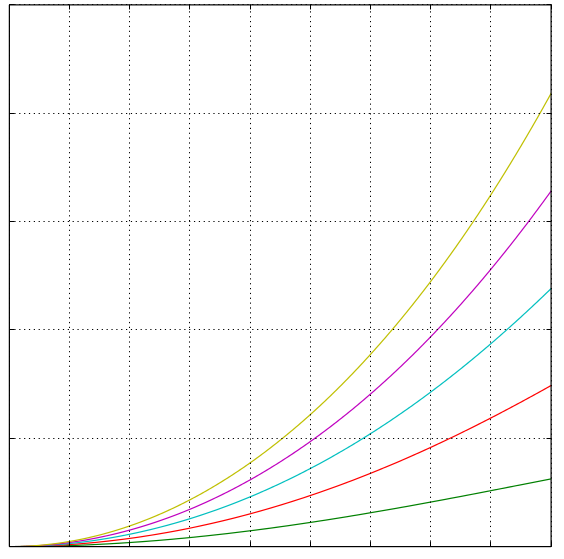
\includegraphics[scale=0.5]{actividad9.png}
\end{center}

Podemos observar que existe una diferencia a la gráfica original, ya que las curvas se encuentran invertidas en su orden. Sin embargo resulta una herramienta útil para conocer el error que se estará cometiendo en cada uno de los casos estudiados y de esta forma se nos permite tener la capacidad de realizar una mejor elección al momento de desarrollar nuestras series; ya que controlaremos el error cometido en los cálculos siendo así nuestro resultados más confiables y adecuados para cada contexto en específico.






\pagebreak







\section*{\textcolor{Purple}{Anexos}}
\subsection*{\textcolor{RubineRed}{Secuencia en Maxima para el periodo del péndulo.}}

\noindent
%%%%%%%%%%%%%%%
%%% INPUT:
\begin{minipage}[t]{8ex}{\color{red}\bf
\begin{verbatim}
(%i3) 
\end{verbatim}}
\end{minipage}
\begin{minipage}[t]{\textwidth}{\color{blue}
\begin{verbatim}
B : taylor((1/sqrt(1-k^2*sin(x)^2)), x, 0, 8);
\end{verbatim}}
\end{minipage}

\noindent
%%%%%%%%%%%%%%%
%%% INPUT:
\begin{minipage}[t]{8ex}{\color{red}\bf
\begin{verbatim}
(%i4) 
\end{verbatim}}
\end{minipage}
\begin{minipage}[t]{\textwidth}{\color{blue}
\begin{verbatim}
i0 : coeff(B,x,0);
\end{verbatim}}
\end{minipage}

\noindent
%%%%%%%%%%%%%%%
%%% INPUT:
\begin{minipage}[t]{8ex}{\color{red}\bf
\begin{verbatim}
(%i5) 
\end{verbatim}}
\end{minipage}
\begin{minipage}[t]{\textwidth}{\color{blue}
\begin{verbatim}
i2 : coeff(B,x,2);
\end{verbatim}}
\end{minipage}

\noindent
%%%%%%%%%%%%%%%
%%% INPUT:
\begin{minipage}[t]{8ex}{\color{red}\bf
\begin{verbatim}
(%i6) 
\end{verbatim}}
\end{minipage}
\begin{minipage}[t]{\textwidth}{\color{blue}
\begin{verbatim}
i4 : coeff(B,x,4);
\end{verbatim}}
\end{minipage}

\noindent
%%%%%%%%%%%%%%%
%%% INPUT:
\begin{minipage}[t]{8ex}{\color{red}\bf
\begin{verbatim}
(%i7) 
\end{verbatim}}
\end{minipage}
\begin{minipage}[t]{\textwidth}{\color{blue}
\begin{verbatim}
i6 : coeff(B,x,6);
\end{verbatim}}
\end{minipage}

\noindent
%%%%%%%%%%%%%%%
%%% INPUT:
\begin{minipage}[t]{8ex}{\color{red}\bf
\begin{verbatim}
(%i8) 
\end{verbatim}}
\end{minipage}
\begin{minipage}[t]{\textwidth}{\color{blue}
\begin{verbatim}
i8 : coeff(B,x,8);
\end{verbatim}}
\end{minipage}

\noindent
%%%%%%%%%%%%%%%
%%% INPUT:
\begin{minipage}[t]{8ex}{\color{red}\bf
\begin{verbatim}
(%i9) 
\end{verbatim}}
\end{minipage}
\begin{minipage}[t]{\textwidth}{\color{blue}
\begin{verbatim}
S : i0 + i2*x^2 + i4*x^4 + i6*x^6 + i8*x^8;
\end{verbatim}}
\end{minipage}

\noindent
%%%%%%%%%%%%%%%
%%% INPUT:
\begin{minipage}[t]{8ex}{\color{red}\bf
\begin{verbatim}
(%i10) 
\end{verbatim}}
\end{minipage}
\begin{minipage}[t]{\textwidth}{\color{blue}
\begin{verbatim}
integrate(S,x);
\end{verbatim}}
\end{minipage}

\noindent
%%%%%%%%%%%%%%%
%%% INPUT:
\begin{minipage}[t]{8ex}{\color{red}\bf
\begin{verbatim}
(%i11) 
\end{verbatim}}
\end{minipage}
\begin{minipage}[t]{\textwidth}{\color{blue}
\begin{verbatim}
integrate(S,x,0,pi/2);
\end{verbatim}}
\end{minipage}

\noindent
%%%%%%%%%%%%%%%
%%% INPUT:
\begin{minipage}[t]{8ex}{\color{red}\bf
\begin{verbatim}
(%i12) 
\end{verbatim}}
\end{minipage}
\begin{minipage}[t]{\textwidth}{\color{blue}
\begin{verbatim}
P : %;
\end{verbatim}}
\end{minipage}

\noindent
%%%%%%%%%%%%%%%
%%% INPUT:
\begin{minipage}[t]{8ex}{\color{red}\bf
\begin{verbatim}
(%i13) 
\end{verbatim}}
\end{minipage}
\begin{minipage}[t]{\textwidth}{\color{blue}
\begin{verbatim}
define(k(%theta),sin(%theta));
\end{verbatim}}
\end{minipage}

\noindent
%%%%%%%%%%%%%%%
%%% INPUT:
\begin{minipage}[t]{8ex}{\color{red}\bf
\begin{verbatim}
(%i14) 
\end{verbatim}}
\end{minipage}
\begin{minipage}[t]{\textwidth}{\color{blue}
\begin{verbatim}
subst(k(%theta/2),k,P);
\end{verbatim}}
\end{minipage}

\noindent
%%%%%%%%%%%%%%%
%%% INPUT:
\begin{minipage}[t]{8ex}{\color{red}\bf
\begin{verbatim}
(%i15) 
\end{verbatim}}
\end{minipage}
\begin{minipage}[t]{\textwidth}{\color{blue}
\begin{verbatim}
F : %;
\end{verbatim}}
\end{minipage}

\noindent
%%%%%%%%%%%%%%%
%%% INPUT:
\begin{minipage}[t]{8ex}{\color{red}\bf
\begin{verbatim}
(%i16) 
\end{verbatim}}
\end{minipage}
\begin{minipage}[t]{\textwidth}{\color{blue}
\begin{verbatim}
F* 2/%pi;
\end{verbatim}}
\end{minipage}

\noindent
%%%%%%%%%%%%%%%
%%% INPUT:
\begin{minipage}[t]{8ex}{\color{red}\bf
\begin{verbatim}
(%i17) 
\end{verbatim}}
\end{minipage}
\begin{minipage}[t]{\textwidth}{\color{blue}
\begin{verbatim}
define(F(%theta), expand(%));
\end{verbatim}}
\end{minipage}

\noindent
%%%%%%%%%%%%%%%
%%% INPUT:
\begin{minipage}[t]{8ex}{\color{red}\bf
\begin{verbatim}
-->  
\end{verbatim}}
\end{minipage}
\begin{minipage}[t]{\textwidth}{\color{blue}
\begin{verbatim}
/*Secuencia correcta*/
B : taylor((1/sqrt(1-k^2*sin(x)^2)), x, 0, 8);
\end{verbatim}}
\end{minipage}

\noindent
%%%%%%%%%%%%%%%
%%% INPUT:
\begin{minipage}[t]{8ex}{\color{red}\bf
\begin{verbatim}
(%i19) 
\end{verbatim}}
\end{minipage}
\begin{minipage}[t]{\textwidth}{\color{blue}
\begin{verbatim}
integrate(B,x,0,%pi/2);
\end{verbatim}}
\end{minipage}

\noindent
%%%%%%%%%%%%%%%
%%% INPUT:
\begin{minipage}[t]{8ex}{\color{red}\bf
\begin{verbatim}
(%i20) 
\end{verbatim}}
\end{minipage}
\begin{minipage}[t]{\textwidth}{\color{blue}
\begin{verbatim}
C : expand(%);
\end{verbatim}}
\end{minipage}

\noindent
%%%%%%%%%%%%%%%
%%% INPUT:
\begin{minipage}[t]{8ex}{\color{red}\bf
\begin{verbatim}
(%i21) 
\end{verbatim}}
\end{minipage}
\begin{minipage}[t]{\textwidth}{\color{blue}
\begin{verbatim}
define(K(%theta),sin(%theta));
\end{verbatim}}
\end{minipage}

\noindent
%%%%%%%%%%%%%%%
%%% INPUT:
\begin{minipage}[t]{8ex}{\color{red}\bf
\begin{verbatim}
(%i22) 
\end{verbatim}}
\end{minipage}
\begin{minipage}[t]{\textwidth}{\color{blue}
\begin{verbatim}
D : subst(K(%theta/2),k,C);
\end{verbatim}}
\end{minipage}

\noindent
%%%%%%%%%%%%%%%
%%% INPUT:
\begin{minipage}[t]{8ex}{\color{red}\bf
\begin{verbatim}
(%i23) 
\end{verbatim}}
\end{minipage}
\begin{minipage}[t]{\textwidth}{\color{blue}
\begin{verbatim}
D * 2/%pi;
\end{verbatim}}
\end{minipage}

\noindent
%%%%%%%%%%%%%%%
%%% INPUT:
\begin{minipage}[t]{8ex}{\color{red}\bf
\begin{verbatim}
(%i24) 
\end{verbatim}}
\end{minipage}
\begin{minipage}[t]{\textwidth}{\color{blue}
\begin{verbatim}
F: expand(%);
\end{verbatim}}
\end{minipage}

\noindent
%%%%%%%%%%%%%%%
%%% INPUT:
\begin{minipage}[t]{8ex}{\color{red}\bf
\begin{verbatim}
(%i25) 
\end{verbatim}}
\end{minipage}
\begin{minipage}[t]{\textwidth}{\color{blue}
\begin{verbatim}
define(T(%theta), (2*%pi)*(sqrt(l/g))*(F));
\end{verbatim}}
\end{minipage}

\noindent
%%%%%%%%%%%%%%%
%%% INPUT:
\begin{minipage}[t]{8ex}{\color{red}\bf
\begin{verbatim}
(%i26) 
\end{verbatim}}
\end{minipage}
\begin{minipage}[t]{\textwidth}{\color{blue}
\begin{verbatim}
l :1;
g :9.8;
float(T(%pi/2));
\end{verbatim}}
\end{minipage}

\noindent
%%%%%%%%%%%%%%%
%%% INPUT:
\begin{minipage}[t]{8ex}{\color{red}\bf
\begin{verbatim}
(%i29) 
\end{verbatim}}
\end{minipage}
\begin{minipage}[t]{\textwidth}{\color{blue}
\begin{verbatim}
kill(all);
\end{verbatim}}
\end{minipage}

\noindent
%%%%%%%%%%%%%%%
%%% INPUT:
\begin{minipage}[t]{8ex}{\color{red}\bf
\begin{verbatim}
(%i1) 
\end{verbatim}}
\end{minipage}
\begin{minipage}[t]{\textwidth}{\color{blue}
\begin{verbatim}
kill(all);
\end{verbatim}}
\end{minipage}

\noindent
%%%%%%%%%%%%%%%
%%% INPUT:
\begin{minipage}[t]{8ex}{\color{red}\bf
\begin{verbatim}
(%i1) 
\end{verbatim}}
\end{minipage}
\begin{minipage}[t]{\textwidth}{\color{blue}
\begin{verbatim}
(1/sqrt(1-k^2*sin(x)^2));
\end{verbatim}}
\end{minipage}

\pagebreak
\begin{thebibliography}{X}
 \bibitem{1} \textsc{Wikipedia, La enciclopedia libre; "Serie de Taylor"; 2016}
 \bibitem{2} \textsc{Wolfram MathWorld; "Mauclarin Series"}
 \bibitem{5} \textsc{Wikipedia, The free encyclopedia; "Pendulum(mathematics)";2016}
\end{thebibliography}
\end{document}